\documentclass[twocoloumn]{article}
\usepackage[utf8]{inputenc}
\usepackage{amssymb}
\usepackage{gensymb}
\usepackage{amsmath}
\usepackage{graphicx}
\usepackage{multicol}
\graphicspath{{figures/}}
\title{AI1110 - Assignment 1}
\author{Kushagra Gupta}

\begin{document}
\maketitle 
\begin{multicols}{2}
\section*{Problem Statement}

\begin{center}
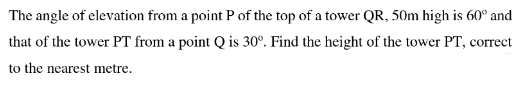
\includegraphics[width=167.5pt]{Q.png}\\
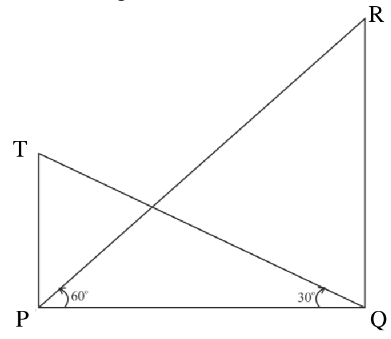
\includegraphics[width=167.5pt]{figure.png}
\end{center}

\section*{Solution}

In $\Delta$PQR, 

$\angle$RPQ  $= 60\degree$ and QR$ = 50$m, using basic trigonometric equation in a right-angled triangle, we know that,

$$\tan(\theta)=\frac{perpendicular}{base}$$

\noindent Hence, 

\begin{align*}
\hspace{60pt}&\tan(\angle RPQ) = \frac{QR}{PQ} \\
&\Rightarrow PQ = \frac{QR}{\tan(\angle RPQ)} \\
&\Rightarrow PQ = \frac{50}{\tan(60\degree)}\, m
\hspace{5pt}[\because \angle RPQ = 60\degree \, \& \, QR = 50m] \\
&\Rightarrow PQ = \frac{50}{\sqrt{3}}\, m \hspace{25pt}-(1)
\end{align*}

Now in $\Delta PQT$, $\angle PQT = 30\degree$.

\begin{align*}
\therefore &\tan(\angle PQT) = \frac{PT}{PQ} \\
&\Rightarrow PT = PQ \times \tan(\angle PQT)\\
&\Rightarrow PT = PQ \times \tan(30 \degree)\\
&\Rightarrow PT = \frac{50}{\sqrt{3}} \times \tan(30 \degree) \, m \hspace{30pt}[using (1)]\\
&\Rightarrow PT = \frac{50}{3}\, m
\end{align*}

\noindent $\therefore$ PT  $ \approx 17 $ metres after rounding off.

\vspace{2pt}
\noindent This can be verified by plotting QR , $\angle RPQ$ and $\angle PQT$ and approximating 
\noindent the length of PT.
\end{multicols}

\pagebreak

\section*{Output}
\noindent The Output of the program used to verify the answer is given below:

\begin{figure}[h]
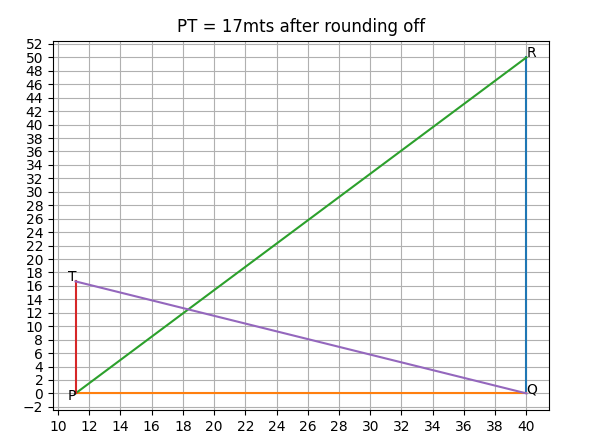
\includegraphics[width=\textwidth]{output.png}
\caption{Plot of the figure and calculated length}

\end{figure}
\end{document}
